\graphicspath{ {../../images/} }
\usetikzlibrary{external}

\title{ICS0026 Cryptography}
\subtitle{Block ciphers \& AES}
\date{\today}
\author{Taaniel Kraavi}
\institute%
{%
  \textit{IT College}\\
  \textit{Tallinn University of Technology}
}

\begin{document}
\begin{frame}
  \titlepage
\end{frame}

\begin{frame}{Block ciphers}
  \begin{center}
  \begin{tikzpicture}
    %\node (f) at ($(2.5cm,0)$) [minimum size=1.25cm,rounded corners=1ex,fill=red!20,draw] {$\ENC$};
    \node (f) at ($(2.5cm,0)$) [minimum size=1.25cm,fill=gray!20,draw] {$\ENC$};
    \node (m) [above of=f, node distance=2cm] {\textit{message}};
    \node (k) [left of=f, node distance=1.5cm] {\textit{key}};
    \node (c) [below of=f, node distance=2cm] {\textit{ciphertext}};

    \node[rectangle, draw, text width=2cm, text height=0.25cm] (mbox)
    [
      below of=m,
      node distance=0.5cm,
      inner sep=0,
      %outer sep=0.1cm,
      path picture={\draw[step=0.25]
        (path picture bounding box.north west)
        grid
        (path picture bounding box.south east);
      }] {};
    \node[rectangle, draw, text width=2cm, text height=0.25cm] (cbox)
    [
      above of=c,
      node distance=0.5cm,
      inner sep=0,
      %outer sep=0.1cm,
      path picture={\draw[step=0.25]
        (path picture bounding box.north west)
        grid
        (path picture bounding box.south east);
    }] {};

    \draw[-latex] (mbox) -- (f);
    \draw[-latex] (k) -- (f);
    \draw[-latex] (f) -- (cbox);
  \end{tikzpicture}
  \hspace*{2cm}
  \begin{tikzpicture}
    %\node (f) at ($(2.5cm,0)$) [minimum size=1.25cm,rounded corners=1ex,fill=red!20,draw] {$\ENC$};
    \node (f) at ($(2.5cm,0)$) [minimum size=1.25cm,fill=gray!20,draw] {$\DEC$};
    \node (c) [above of=f, node distance=2cm] {\textit{ciphertext}};
    \node (k) [left of=f, node distance=1.5cm] {\textit{key}};
    \node (m) [below of=f, node distance=2cm] {\textit{message}};

    \node[rectangle, draw, text width=2cm, text height=0.25cm] (cbox)
    [
      below of=c,
      node distance=0.5cm,
      inner sep=0,
      %outer sep=0.1cm,
      path picture={\draw[step=0.25]
        (path picture bounding box.north west)
        grid
        (path picture bounding box.south east);
      }] {};
    \node[rectangle, draw, text width=2cm, text height=0.25cm] (mbox)
    [
      above of=m,
      node distance=0.5cm,
      inner sep=0,
      %outer sep=0.1cm,
      path picture={\draw[step=0.25]
        (path picture bounding box.north west)
        grid
        (path picture bounding box.south east);
    }] {};

    \draw[-latex] (cbox) -- (f);
    \draw[-latex] (k) -- (f);
    \draw[-latex] (f) -- (mbox);
  \end{tikzpicture}
  \end{center}

  \pause
  Properties:
  \begin{itemize}[<+->]
    \item Messages and ciphertexts of fixed size (blocks)
    \item Deterministic by default
    \item Confusion \& diffusion
  \end{itemize}
\end{frame}

\begin{frame}{Modes of operation}
  Different \emph{modes of operation} are used to extend operations to data larger than a block.

  \pause
  Examples:
  \begin{itemize}[<+->]
    \item ECB (NB! danger-zone)
    \item CBC
    \item CTR
    \item GCM (authenticated encryption)
  \end{itemize}

  \pause
  Warnings:
  \begin{itemize}[<+->]
    \item A secure cipher with an insecure mode is insecure!
    \item Pick the right mode for the right task!
  \end{itemize}  
\end{frame}

\begin{frame}{Electronic Codebook (ECB) mode}
  \begin{center}
  \begin{tikzpicture}
    \foreach \x in {1, 2, 3} {
      \node (f\x) at ($\x*(2.5cm,0)$) [minimum size=1.25cm,fill=gray!20,draw] {$\ENC$};
      \node (m\x) [above of=f\x, node distance=1.5cm] {$m_\x$};
      \node (k\x) [left of=f\x, node distance=1.5cm] {$k$};
      \node (c\x) [below of=f\x, node distance=1.5cm] {$c_\x$};

      \draw[-latex] (m\x) -- (f\x);
      \draw[-latex] (k\x) -- (f\x);
      \draw[-latex] (f\x) -- (c\x);
    }
  \end{tikzpicture}
  \end{center}

  \pause
  Do not use, \emph{ever}\textsuperscript{*}.

  \pause
  A building block for
  \begin{itemize}[<+->]
    \item more complex modes
    \item other cryptographic constructions
  \end{itemize}
\end{frame}

\begin{frame}{ECB Tux}
  \begin{columns}
    \begin{column}{0.5\textwidth}
      \begin{center}
        
\includegraphics[width=150px]{tux}
      \end{center}
    \end{column}
    \begin{column}{0.5\textwidth}
      \pause
      \begin{center}
        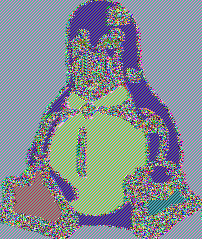
\includegraphics[width=150px]{tux_ecb}
      \end{center}
    \end{column}
  \end{columns}
\end{frame}

\begin{frame}{Initialisation Vector (IV)}
  \begin{center}
  \begin{tikzpicture}
    \foreach \x in {1, 2, 3} {
      \node (f\x) at ($\x*(2.5cm,0)$) [minimum size=1.25cm,fill=gray!20,draw] {$\ENC$};
      \node (p\x) [above of=f\x, node distance=1.5cm, circle, draw] {};
      \node (m\x) [above of=p\x, node distance=1cm] {$m_\x$};
      \node (k\x) [left of=f\x, node distance=1.5cm] {$k$};
      \node (c\x) [below of=f\x, node distance=1.5cm] {$c_\x$};

      \draw[-] (p\x.east) -- (p\x.west);

      \draw[-latex] (m\x) -- (f\x);
      \draw[-latex] (k\x) -- (f\x);
      \draw[-latex] (f\x) -- (c\x);

      \node (iv\x) [left of=p\x, node distance=1.5cm] {$IV_\x$};
      \draw[-latex] (iv\x) -- (p\x);
    }
  \end{tikzpicture}
  \end{center}

  \begin{itemize}[<+(1)->]
    \item Different ways to apply the IV (XOR on the figure)
    \item Do not reuse (under the same key)
    \item Not secret: sent with the ciphertext
  \end{itemize}
\end{frame}

\begin{frame}{Cipher Block Chaining (CBC) mode}
  \begin{center}
  \begin{tikzpicture}
    \foreach \x in {1, 2, 3} {
      \node (f\x) at ($\x*(2.5cm,0)$) [minimum size=1.25cm,fill=gray!20,draw] {$\ENC$};
      \node (p\x) [above of=f\x, node distance=1.5cm, circle, draw] {};
      \node (m\x) [above of=p\x, node distance=1cm] {$m_\x$};
      \node (k\x) [left of=f\x, node distance=1.5cm] {$k$};
      \node (c\x) [below of=f\x, node distance=1.5cm] {$c_\x$};

      \draw[-] (p\x.east) -- (p\x.west);

      \draw[-latex] (m\x) -- (f\x);
      \draw[-latex] (k\x) -- (f\x);
      \draw[-latex] (f\x) -- (c\x);
    }

    \node (iv) [left of=p1, node distance=2cm] {$IV$};
    \draw[-latex] (iv) -- (p1);

    \node (c0) [left of=c1, node distance=2cm] {$c_0$};
    \draw[-latex] (iv) -- (c0);

    \foreach \x in {1, 2} {
        \draw[-latex] ($(c\x) + (0,0.6cm)$) -| +(0.8cm,2.4cm) -- ($(p\the\numexpr\x+1\relax.west)$);
    }
  \end{tikzpicture}
  \end{center}

  \begin{columns}
    \begin{column}{0.5\textwidth}
      \begin{itemize}[<+(1)->]
        \item Serial encryption
        \item Parallel decryption
        \item Pre-encryption change propagation
    \end{itemize}
    \end{column}
    \begin{column}{0.5\textwidth}
      \pause
      \begin{block}{Note}
        Not security properties!
      \end{block}
    \end{column}
  \end{columns}
\end{frame}

\begin{frame}{CBC Tux}
  \begin{columns}
    \begin{column}{0.5\textwidth}
      \begin{center}
        
\includegraphics[width=150px]{tux}
      \end{center}
    \end{column}
    \begin{column}{0.5\textwidth}
      \pause
      \begin{center}
        
\includegraphics[width=150px]{tux_secure}
      \end{center}
    \end{column}
  \end{columns}
\end{frame}

\begin{frame}
  \frametitle{Counter (CTR) mode}

  \begin{center}
  \begin{tikzpicture}
    \node (f1) at ($(2.5cm,0)$) [minimum size=1.25cm,fill=gray!20,draw] {$\ENC$};
    \node (n1) [above of=f1, node distance=1.5cm] {$nc$, $ctr$};
    \node (k1) [left of=f1, node distance=1.5cm] {$k$};
    \node (c1) [below of=f1, node distance=2.5cm] {$c_1$};
    \node (p1) [below of=f1, node distance=1.5cm, circle, draw] {};
    \node (m1) [left of=p1, node distance=1cm] {$m_1$};

    \draw[-] (p1.east) -- (p1.west);

    \draw[-latex] (n1) -- (f1);
    \draw[-latex] (m1) -- (p1);
    \draw[-latex] (k1) -- (f1);
    \draw[-latex] (f1) -- (c1);

    \foreach \x in {2, 3} {
      \node (f\x) at ($\x*(2.5cm,0)$) [minimum size=1.25cm,fill=gray!20,draw] {$\ENC$};
      \node (n\x) [above of=f\x, node distance=1.5cm] {$nc$, $ctr+\the\numexpr\x-1$};
      \node (k\x) [left of=f\x, node distance=1.5cm] {$k$};
      \node (c\x) [below of=f\x, node distance=2.5cm] {$c_\x$};
      \node (p\x) [below of=f\x, node distance=1.5cm, circle, draw] {};
      \node (m\x) [left of=p\x, node distance=1cm] {$m_\x$};

      \draw[-] (p\x.east) -- (p\x.west);

      \draw[-latex] (n\x) -- (f\x);
      \draw[-latex] (m\x) -- (p\x);
      \draw[-latex] (k\x) -- (f\x);
      \draw[-latex] (f\x) -- (c\x);
    }
  \end{tikzpicture}
  \end{center}

  \begin{itemize}[<+(1)->]
    \item Operates as a stream cipher
    \item The \emph{nonce} is like the IV: never reuse it for the same key
    \item Counter combined using an \emph{invertible} operation, e.g. $\oplus$, $||$
    \item Prefer $||$ due to counter pitfalls! (e.g. non-random nonces)
  \end{itemize}
\end{frame}

\begin{frame}{Authenticated encryption (AE)}
  \begin{block}{Note}
    We will cover data authentication \& integrity in a later lecture.
  \end{block}

  \vspace*{1em}

  \begin{columns}[b]
    \begin{column}{0.4\textwidth}
      \pause
      AE assures:
      \begin{itemize}[<+->]
        \item confidentiality
        \item authenticity
      \end{itemize}
    \end{column}
    \begin{column}{0.53\textwidth}
      \pause
      Authenticity is a special case of integrity.
    \end{column}
  \end{columns}

  \vspace*{1em}

  \pause
  Authenticated encryption with associated data (AEAD):
  \begin{itemize}[<+->]
    \item Additional associated data AAD: the \emph{header}
    \item Authenticated, but not confidential
  \end{itemize}

  \vspace*{1em}

  \pause
  Authenticity provided by the \emph{authentication tag}.
\end{frame}

\begin{frame}
  \frametitle{Galois/Counter (GCM) mode}

  You do not need to understand this!
  \begin{center}
    \url{https://csrc.nist.rip/groups/ST/toolkit/BCM/documents/proposedmodes/gcm/gcm-spec.pdf\#page=8}
  \end{center}
  \pause
  Only what it does (not how) and why it is useful.
\end{frame}

\begin{frame}{Dangers of GCM}
  In GCM-mode, nonce reuse enables the \emph{forbidden attack}:
  \begin{itemize}[<+(1)->]
    \item practical attack (real-world applicable)
    \item enables message forgery (breaks authenticity)
  \end{itemize}

  \pause
  How can we protect against nonce reuse?

  \pause
  SIV mode:
  \begin{itemize}[<+->]
    \item Synthetic initialization vector
    \item \href{https://datatracker.ietf.org/doc/html/rfc5297}{RFC 5297}
    \item Example: AES-GCM-SIV (\href{https://datatracker.ietf.org/doc/html/rfc8452}{RFC 8452})
  \end{itemize}
\end{frame}

\begin{frame}{Padding messages}
  How should we pad messages?

  \begin{columns}
    \begin{column}{0.5\textwidth}
      \begin{itemize}[<+(1)->]
        \item Zero padding\\
        \texttt{1a 1a 1a 1a 1a 00 00 00}
        \item ISO/IEC 7816-4\\
        \texttt{1a 1a 1a 1a 1a 80 00 00}
        \item PKCS\#5 and PKCS\#7\\
        \texttt{1a 1a 1a 1a 1a 03 03 03}\\
        \texttt{1a 1a 1a 05 05 05 05 05}
      \end{itemize}
    \end{column}
    \begin{column}{0.5\textwidth}
      \begin{itemize}[<+(1)->]
        \item ANSI X9.23 (withdrawn)\\
        \texttt{1a 1a 1a 1a 1a 00 00 03}
        \item ISO 10126 (withdrawn)\\
        \texttt{1a 1a 1a 1a 1a 81 A6 03}
      \end{itemize}
    \end{column}
  \end{columns}

  \vspace*{1em}

  \pause
  Padding is always added.
\end{frame}

\begin{frame}{Block-size \& key size}
  A block cipher may have different parameters for the \enquote{same} cipher.

  \pause
  Block size:
  \begin{itemize}
    \item The number of bits in a block, i.e. message/ciphertext length
    \pause
    \item Typical values are: 64 (bad), 128, 192, 256 bits
  \end{itemize}

  \pause
  Key length:
  \begin{itemize}
    \item Usually tied to the \enquote{strength} of the cipher
    \pause
    \item Typical values are: 128, 192, 256 bits
  \end{itemize}

  \pause
  More complex parameters exist, but usually are not of the user's concern.
\end{frame}

\begin{frame}{Security level}
  \pause
  The \emph{security level} is a measure of the \enquote{strength} that a cryptographic primitive achieves.

  \begin{itemize}[<+(1)->]
    \item Often called \emph{bits of security}
    \item $n$-bits of security: $2^n$ operations to break (typical definition)
    \item Essentially refers to the \emph{brute-force} break
    \item Not always clear cut!
  \end{itemize}
\end{frame}

\begin{frame}{Security level}
  \begin{itemize}[<+->]
    \item Secure symmetric cryptosystems: classical strength = key size (typically)
    \item Strength measured differently for different primitives
    \item Broken primitive: an attack beats the \emph{target security level}
    \item Not all \emph{breaks} are practical
    \item \enquote{Practical} break historically fixed at $2^{80}$ ($2^{100}$ also common) \dots
    \item \dots{}but is arguably no longer enough
    \item Bitcoin hashing data: \url{https://www.blockchain.com/explorer/charts/hash-rate}
  \end{itemize}
\end{frame}

\begin{frame}{Some ciphers}
  Some well-known ciphers include
  \pause
  \begin{itemize}[<+->]
    \item DES (Data Encryption Standard): belongs in a museum, weak!
    \item 3DES: deprecated
    \item Twofish: successor to the insecure Blowfish
    \item RC5 (\& RC6): used to be patented
    \item Camellia, Serpent, ARIA, \dots
    \item AES (Advanced Encryption Standard): sometimes called the \enquote{gold standard}
  \end{itemize}

  \vspace*{1em}

  \pause
  Block ciphers seem (and are) more \enquote{popular}.
  \begin{itemize}[<+(1)->]
    \item historical reasons, e.g. perception (RC4) \& standardisation
    \item \enquote{better} to implement in hardware (less so these days)
    \item versatility
  \end{itemize}
\end{frame}

\begin{frame}{AES}
  Advanced Encryption Standard
  \begin{itemize}[<+(1)->]
    \item Originally called Rijndael
    \item Standardised by NIST in 2001 (\href{https://csrc.nist.gov/pubs/fips/197/final}{FIPS 197})
    \item Later standardised by ISO (\href{https://www.iso.org/standard/54531.html}{ISO/IEC 18033-3:2010})
    \item Superseded the Data Encryption Standard (DES)
  \end{itemize}

  \pause
  Practical info:
  \begin{itemize}[<+->]
    \item Block size: 128 bits
    \item Key sizes: 128, 192, 256 bits
  \end{itemize}
\end{frame}

\begin{frame}{Attacks on AES}
  No current practical attack can break AES confidentiality (when correctly used and implemented).

  \begin{itemize}[<+(1)->]
    \item Best current key recovery attack: $2^{126.0}$ operations
    \item Security can be weakened by the mode of operation
    \item Lots of problematic implementations (side channel attacks)
    \item Various breaks if not enough \emph{rounds} are performed
    \item AES-256 is considered \emph{quantum resistant} (128 bits of security)
    \item AES-128, AES-192 are not considered quantum resistant
  \end{itemize}

  \pause
  Pick the implementation and parameters carefully!
\end{frame}

\begin{frame}{Block ciphers vs stream ciphers}
  Block ciphers:
  \begin{itemize}[<+(1)->]
    \item Well suited for static/fixed data, e.g. stored files, passwords, \dots
    \item Often used for \enquote{regular} communication, e.g. messaging apps (WhatsApp, Signal)
    \item Can work as stream ciphers
    \item Typically better studied
    \item Hardware acceleration (AES)
  \end{itemize}

  \pause
  Stream ciphers:
  \begin{itemize}[<+(1)->]
    \item Well suited for data streams, e.g. real-time communication, internet traffic
    \item Modern stream ciphers are very fast (efficient in software)
    \item Redundancy for block-cipher breaks (for pure stream ciphers)
  \end{itemize}

  \pause
  Neither (typically) provides data authentication by default!
\end{frame}

\begin{frame}{ChaCha20 vs AES}
  \pause
  Not going to tell you $>$:)
  \begin{itemize}[<+(1)->]
    \item You are generally fine regardless of which you pick.
    \item For web-servers, you should support both!
  \end{itemize}

  \pause
  Things to keep in mind:
  \begin{itemize}[<+(1)->]
    \item Performance: which is faster for you? your peers/use case?
    \item Standardisation: AES-GCM is FIPS compliant, ChaCha20 is not
    \item Implementation quality: ChaCha20 is timing safe (not the whole story!)
    \item Degree of authenticity: (X)ChaCha20-Poly1305 offers stronger properties
    \item Theoretical security: ChaCha20 has a larger security \enquote{margin}
  \end{itemize}
\end{frame}

\begin{frame}{Built using block ciphers}
  \begin{itemize}[<+(1)->]
    \item Stream ciphers
    \item CSPRNGs
    \item Cryptographic hash functions
    \item Secure PRPs (pseudo-random permutations)
    \item Message authentication codes (MACs) \& AE
  \end{itemize}
\end{frame}

\begin{frame}{Disk encryption}
  Specific modes of operation exist, e.g. XTS (XTS-AES is standardised).

  \pause
  How to do it with CBC?
  \begin{itemize}[<+(1)->]
    \item Encrypt each sector
    \item Use sector number as IV
    \item ESSIV mode improves it a little (SN + key hash)
    \item No integrity!
  \end{itemize}

  \pause
  Some tools:
  \begin{itemize}[<+(1)->]
    \item LUKS (dm-crypt)
    \item BitLocker
    \item FileVault
  \end{itemize}

  \pause
  Trivia: Google Adiantum cipher composition.
\end{frame}

\begin{frame}{Keys and passwords}
  \begin{block}{Note}
    We will cover hash functions \& key derivation again in a later lecture.
  \end{block}

  \pause
  A human-generated password typically has low \emph{entropy}, i.e. it is not random enough.

  \pause
  Key derivation functions
  \begin{itemize}[<+(1)->]
    \item Derive secret keys from a secret value
    \item \enquote{Stretches} (and strengthens) secrets
    \item Hash-function or block-cipher based (typically)
    \item Attack resistant: slow down attacks
  \end{itemize}

  \pause
  Encryption keys are derived from passwords for \enquote{user-facing} symmetric cryptosystems.
\end{frame}

\end{document}
